% ---------------------------------------------------------------
% GATE EC 2025 -- single-file version (preamble, macros, figures, questions)
% (article class + Times, because IEEEtran.cls is not available in
%  the build environment; problems.tex itself is class-independent)
% ---------------------------------------------------------------
\documentclass[12pt,a4paper]{article}
\usepackage[margin=2.2cm]{geometry}
\usepackage{mathptmx}                 % Times text + math
\usepackage{amsmath,amssymb,mathtools}
\usepackage{enumitem}
\usepackage{multicol}
\usepackage{float}                    % [H] placement
\usepackage{chngcntr}
\usepackage{graphicx}
\usepackage{xcolor}
\usepackage{listings}
\usepackage{tikz}
\usetikzlibrary{arrows.meta,calc,positioning,fit,patterns,shapes.geometric,circuits.logic.US}
\usepackage[american]{circuitikz}
\usepackage[colorlinks=true,allcolors=red,hypertexnames=false]{hyperref}

% ---------------------------------------------------------------
% macros.tex : every custom macro used by problems.tex
% (If your own book preamble already defines these, you do NOT
%  need this file -- use it only for the stand-alone preview.)
% ---------------------------------------------------------------
\providecommand{\pr}[1]{\Pr\left(#1\right)}
\providecommand{\brak}[1]{\left(#1\right)}
\providecommand{\sbrak}[1]{\left[#1\right]}
\providecommand{\cbrak}[1]{\left\{#1\right\}}
\providecommand{\abs}[1]{\left\lvert#1\right\rvert}
\providecommand{\rabs}[1]{\left.#1\right\rvert}
\providecommand{\norm}[1]{\left\lVert#1\right\rVert}
\providecommand{\myvec}[1]{\begin{bmatrix}#1\end{bmatrix}}
\providecommand{\mydet}[1]{\left\lvert#1\right\rvert}
\providecommand{\rank}{\operatorname{rank}}
\providecommand{\perm}[2]{{}^{#1}P_{#2}}
\providecommand{\rect}{\operatorname{rect}}
\providecommand{\system}[1]{\xleftrightarrow{\mathcal{#1}}}
\providecommand{\solution}{\noindent\textbf{Solution: }}
\providecommand{\figref}[1]{Fig.~\ref{#1}}
\providecommand{\ang}[1]{\angle #1^{\circ}}
\renewcommand{\j}{\mathrm{j}}
\renewcommand{\vec}[1]{\mathbf{#1}}


% option labels  i)  ii)  iii)  iv)   (second-level enumerate)
\renewcommand{\labelenumii}{\roman{enumii})}
\setlist[enumerate,2]{itemsep=2pt,topsep=3pt}

% equation / figure numbers :  section.subsection.item.k   e.g. 1.2.14.1
% (enumitem's  ref=\thesubsection.\theenumi  already makes \theenumi = 1.2.14)
\counterwithin*{equation}{enumi}
\counterwithin*{figure}{enumi}
\renewcommand{\theequation}{\theenumi.\arabic{equation}}
\renewcommand{\thefigure}{\theenumi.\arabic{figure}}
\renewcommand{\figurename}{Fig.}

\lstset{frame=single,basicstyle=\rmfamily,columns=fullflexible}
\setlength{\parindent}{0pt}

\title{GATE EC 2025}
\author{}
\date{}

\begin{document}
\maketitle
\tableofcontents
\newpage

\section{GATE EC 2025}
\subsection{Formulae}
% ---------------------------------------------------------------
% formulae.tex  --  (empty for now; add formulae LATER)
% Use exactly the same pattern as problems.tex, e.g.
%
% \begin{enumerate}[label=\thesubsection.\arabic*, ref=\thesubsection.\theenumi]
% \item The Laplace transform is defined as
% \begin{align}
% g\brak{t} \system{L} G(s) = \int_{0}^{\infty} e^{-st} g\brak{t}\, dt
% \label{eq:EC25-Laplace-def}
% \end{align}
% \solution (optional derivation)
% ...
% \end{enumerate}
% Then, in any solution, refer to it with \eqref{eq:EC25-Laplace-def}.
% ---------------------------------------------------------------
\noindent\textit{Formulae will be added here.}


\subsection{Problems}
\begin{enumerate}[label=\thesubsection.\arabic*, ref=\thesubsection.\theenumi]
%--------------------------------------------------------------- Q11
\item
Consider the matrix $\vec{A}$ below:
\begin{align}
\vec{A} = \myvec{
2 & 3 & 4 & 5 \\
0 & 6 & 7 & 8 \\
0 & 0 & \alpha & \beta \\
0 & 0 & 0 & \gamma
}
\end{align}
For which of the following combinations of $\alpha$, $\beta$, and $\gamma$, is the rank of $\vec{A}$ at least three?
\hfill (EC~2025)
\begin{enumerate}[label=(\roman*), itemsep=0pt, topsep=2pt]
    \item $\alpha = 0$ and $\beta = \gamma \neq 0$.
    \item $\alpha = \beta = \gamma = 0$.
    \item $\beta = \gamma = 0$ and $\alpha \neq 0$.
    \item $\alpha = \beta = \gamma \neq 0$.
\end{enumerate}
\begin{enumerate}
	\begin{multicols}{2}
    \item Only (i), (iii), and (iv)
    \item Only (iv)
    \item Only (ii)
    \item Only (i) and (iii)
	\end{multicols}
\end{enumerate}

%--------------------------------------------------------------- Q12
\item
Consider the following series:
\begin{enumerate}[label=(\roman*), itemsep=0pt, topsep=2pt]
    \item $\displaystyle\sum_{n=1}^{\infty} \frac{1}{\sqrt{n}}$
    \item $\displaystyle\sum_{n=1}^{\infty} \frac{1}{n\brak{n+1}}$
    \item $\displaystyle\sum_{n=1}^{\infty} \frac{1}{n!}$
\end{enumerate}
Choose the correct option.
\hfill (EC~2025)
\begin{enumerate}
	\begin{multicols}{2}
    \item Only (ii) converges
    \item Only (ii) and (iii) converge
    \item Only (iii) converges
    \item All three converge
	\end{multicols}
\end{enumerate}

%--------------------------------------------------------------- Q13
\item
A pot contains two red balls and two blue balls. Two balls are drawn from this pot randomly without replacement.

What is the probability that the two balls drawn have different colours?
\hfill (EC~2025)
\begin{enumerate}
	\begin{multicols}{4}
    \item $\dfrac{2}{3}$
    \item $\dfrac{1}{3}$
    \item $\dfrac{1}{2}$
    \item $1$
	\end{multicols}
\end{enumerate}

%--------------------------------------------------------------- Q14
\item
Consider a frequency-modulated (FM) signal
\begin{align}
f\brak{t} = A_c \cos\brak{2\pi f_c t + 3\sin\brak{2\pi f_1 t} + 4\sin\brak{6\pi f_1 t}},
\end{align}
where $A_c$ and $f_c$ are, respectively, the amplitude and frequency (in Hz) of the carrier waveform. The frequency $f_1$ is in Hz, and assume that $f_c > 100 f_1$.

The peak frequency deviation of the FM signal in Hz is \underline{\hspace{1cm}}.
\hfill (EC~2025)
\begin{enumerate}
	\begin{multicols}{4}
    \item $15 f_1$
    \item $12 f_1$
    \item $4 f_1$
    \item $2 f_1$
	\end{multicols}
\end{enumerate}

%--------------------------------------------------------------- Q17
\item
Consider the discrete-time system below with input $x[n]$ and output $y[n]$. In the figure, $h_1[n]$ and $h_2[n]$ denote the impulse responses of LTI Subsystems 1 and 2, respectively. Also, $\delta[n]$ is the unit impulse, and $b > 0$.

Assuming $h_2[n] \neq \delta[n]$, the overall system (denoted by the dashed box) is \underline{\hspace{1cm}}.
\hfill (EC~2025)
\begin{enumerate}
	\begin{multicols}{2}
    \item linear and time invariant
    \item linear and time variant
    \item nonlinear and time invariant
    \item nonlinear and time variant
	\end{multicols}
\end{enumerate}
\begin{figure}[H]
\begin{center}
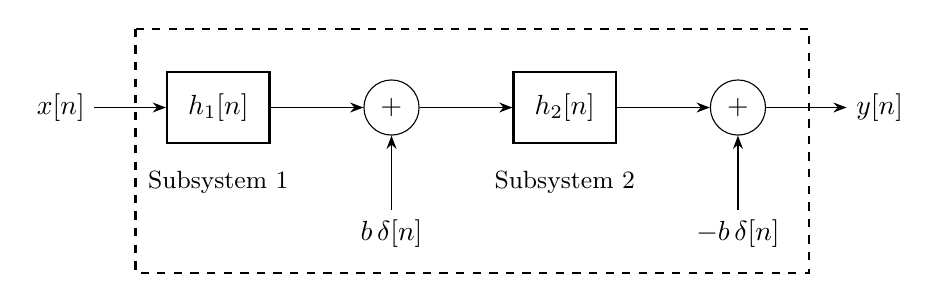
\begin{tikzpicture}[>=Stealth, blk/.style={draw,thick,minimum width=1.3cm,minimum height=0.9cm}, sm/.style={draw,circle,inner sep=0pt,minimum size=0.7cm}]
\node (x) at (0,0) {$x[n]$};
\node[blk] (h1) at (2,0) {$h_1[n]$};
\node[sm] (s1) at (4.2,0) {$+$};
\node[blk] (h2) at (6.4,0) {$h_2[n]$};
\node[sm] (s2) at (8.6,0) {$+$};
\node (y) at (10.4,0) {$y[n]$};
\draw[->] (x)--(h1); \draw[->] (h1)--(s1); \draw[->] (s1)--(h2);
\draw[->] (h2)--(s2); \draw[->] (s2)--(y);
\node (b1) at (4.2,-1.6) {$b\,\delta[n]$}; \draw[->] (b1)--(s1);
\node (b2) at (8.6,-1.6) {$-b\,\delta[n]$}; \draw[->] (b2)--(s2);
\node[font=\small] at (2.0,-0.95) {Subsystem 1};
\node[font=\small] at (6.4,-0.95) {Subsystem 2};
\draw[dashed,thick] (0.95,1.0) rectangle (9.5,-2.1);
\end{tikzpicture}

    \caption{Discrete-time system}
    \label{fig:EC25-17}
\end{center}
\end{figure}

%--------------------------------------------------------------- Q18
\item
Consider a continuous-time, real-valued signal $f\brak{t}$ whose Fourier transform
\begin{align}
F\brak{\omega} = \int_{-\infty}^{\infty} f\brak{t} \exp\brak{-\j \omega t}\, dt
\end{align}
exists.

Which one of the following statements is always TRUE?
\hfill (EC~2025)
\begin{enumerate}
	\begin{multicols}{2}
    \item $\abs{F\brak{\omega}} \leq \displaystyle\int_{-\infty}^{\infty} \abs{f\brak{t}}\, dt$
    \item $\abs{F\brak{\omega}} > \displaystyle\int_{-\infty}^{\infty} \abs{f\brak{t}}\, dt$
    \item $\abs{F\brak{\omega}} \leq \displaystyle\int_{-\infty}^{\infty} f\brak{t}\, dt$
    \item $\abs{F\brak{\omega}} \geq \displaystyle\int_{-\infty}^{\infty} f\brak{t}\, dt$
	\end{multicols}
\end{enumerate}

%--------------------------------------------------------------- Q20
\item
Let $i_C$, $i_L$, and $i_R$ be the currents flowing through the capacitor, inductor, and resistor, respectively, in the circuit given below. The AC admittances are given in Siemens (S).

Which one of the following is TRUE?
\hfill (EC~2025)
\begin{enumerate}
    \item $i_C = 0.25\ang{180}$ A, \; $i_L = 0.1\ang{0}$ A, \; $i_R = 0.2\ang{90}$ A
    \item $i_C = 4\ang{180}$ A, \; $i_L = 10\ang{0}$ A, \; $i_R = 5\ang{90}$ A
    \item $i_C = 0.25\ang{270}$ A, \; $i_L = 0.1\ang{90}$ A, \; $i_R = 0.2\ang{90}$ A
    \item $i_C = 4\ang{90}$ A, \; $i_L = 10\ang{270}$ A, \; $i_R = 5\ang{0}$ A
\end{enumerate}
\begin{figure}[H]
\begin{center}
\begin{circuitikz}[american, scale=0.95, transform shape]
\draw (0,0) to[sV, l=$1\angle 90^\circ$ V] (0,3) -- (8.5,3);
\draw (0,0) -- (8.5,0);
\draw (3.3,3) to[C, l=$j0.25$ S, i=$i_C$] (3.3,0);
\draw (5.6,3) to[L, l=$-j0.1$ S, i=$i_L$] (5.6,0);
\draw (8.5,3) to[R, l=$0.2$ S, i=$i_R$] (8.5,0);
\fill (3.3,3) circle(2pt) (5.6,3) circle(2pt) (3.3,0) circle(2pt) (5.6,0) circle(2pt);
\node at (0.45,2.35) {$+$}; \node at (0.45,0.65) {$-$};
\end{circuitikz}

    \caption{Parallel RLC circuit}
    \label{fig:EC25-20}
\end{center}
\end{figure}

%--------------------------------------------------------------- Q23
\item
A 3-input majority logic gate has inputs $X$, $Y$, and $Z$. The output $F$ of the gate is logic `1' if two or more of the inputs are logic `1'. The output $F$ is logic `0' if two or more of the inputs are logic `0'.

Which one of the following options is a Boolean expression of the output $F$?
\hfill (EC~2025)
\begin{enumerate}
	\begin{multicols}{4}
    \item $XY + YZ + ZX$
    \item $X \oplus Y \oplus Z$
    \item $X + Y + Z$
    \item $XYZ$
	\end{multicols}
\end{enumerate}

%--------------------------------------------------------------- Q24
\item
A full adder and an XOR gate are used to design a digital circuit with inputs $X$, $Y$, and $Z$, and output $F$, as shown below. The input $Z$ is connected to the carry-in input of the full adder.

If the input $Z$ is set to logic `1', then the circuit functions as \underline{\hspace{1cm}} with $X$ and $Y$ as inputs.
\hfill (EC~2025)
\begin{enumerate}
	\begin{multicols}{2}
    \item an adder
    \item a subtractor
    \item a multiplier
    \item a binary to Gray code converter
	\end{multicols}
\end{enumerate}
\begin{figure}[H]
\begin{center}
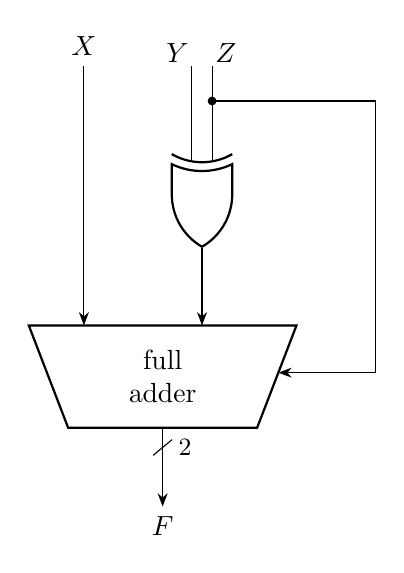
\begin{tikzpicture}[>=Stealth]
% full adder (trapezium)
\draw[thick] (-1.7,0) -- (1.7,0) -- (1.2,-1.3) -- (-1.2,-1.3) -- cycle;
\node[align=center] at (0,-0.65) {full\\adder};
% X input
\node[above] at (-1.0,3.3) {$X$};
\draw[->] (-1.0,3.3) -- (-1.0,0);
% XOR gate pointing down
\node[xor gate US, draw, thick, rotate=-90, logic gate inputs=nn, scale=1.3] (g) at (0.5,1.6) {};
\draw[->] (g.output) -- (g.output |- 0,0);
\node[above left,inner sep=1pt] at (g.input 2 |- 0,3.3) {$Y$};
\node[above right,inner sep=1pt] at (g.input 1 |- 0,3.3) {$Z$};
\draw (g.input 2 |- 0,3.3) -- (g.input 2);
\draw (g.input 1 |- 0,3.3) -- (g.input 1);
% Z also goes to the carry-in
\fill (g.input 1 |- 0,2.85) circle(1.6pt);
\draw (g.input 1 |- 0,2.85) -| (2.7,-0.6);
\draw[->] (2.7,-0.6) -- (1.47,-0.6);
% output F (2 bits)
\draw[->] (0,-1.3) -- (0,-2.3) node[below] {$F$};
\draw (-0.12,-1.65) -- (0.12,-1.45); \node[right,font=\small] at (0.08,-1.55) {2};
\end{tikzpicture}

    \caption{Full adder with XOR gate}
    \label{fig:EC25-24}
\end{center}
\end{figure}

%--------------------------------------------------------------- Q25
\item
Consider the function $f: \mathbb{R} \to \mathbb{R}$, defined as
\begin{align}
f\brak{x} = 2x^3 - 3x^2 - 12x + 1.
\end{align}
Which of the following statements is/are correct?

(Here, $\mathbb{R}$ is the set of real numbers.)
\hfill (EC~2025)
\begin{enumerate}
	\begin{multicols}{2}
    \item $f$ has no global maximizer
    \item $f$ has no global minimizer
    \item $x = -1$ is a local minimizer of $f$
    \item $x = 2$ is a local maximizer of $f$
	\end{multicols}
\end{enumerate}

%--------------------------------------------------------------- Q26
\item
Consider the unity-negative-feedback system shown in \figref{fig:EC25-26a} below, where gain $K \geq 0$. The root locus of this system is shown in \figref{fig:EC25-26b} below.

For what value(s) of $K$ will the system in \figref{fig:EC25-26a} have a pole at $-1 + \j 1$?
\hfill (EC~2025)
\begin{enumerate}
	\begin{multicols}{2}
    \item $K = 5$
    \item $K = \dfrac{1}{5}$
    \item For no positive value of $K$
    \item For all positive values of $K$
	\end{multicols}
\end{enumerate}
\begin{figure}[H]
\begin{center}
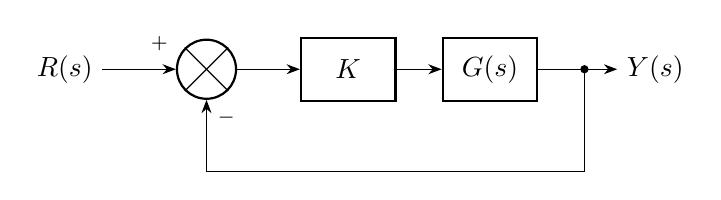
\begin{tikzpicture}[>=Stealth, blk/.style={draw,thick,minimum width=1.2cm,minimum height=0.8cm}]
\node (r) at (0,0) {$R(s)$};
\node[draw,thick,circle,inner sep=0pt,minimum size=0.75cm] (s) at (1.8,0) {};
\draw (s.north west)--(s.south east); \draw (s.north east)--(s.south west);
\node[font=\scriptsize] at (1.2,0.32) {$+$}; \node[font=\scriptsize] at (2.05,-0.62) {$-$};
\node[blk] (k) at (3.6,0) {$K$};
\node[blk] (g) at (5.4,0) {$G(s)$};
\node (y) at (7.5,0) {$Y(s)$};
\draw[->] (r)--(s); \draw[->] (s)--(k); \draw[->] (k)--(g); \draw[->] (g)--(y);
\draw[->] (6.6,0) -- (6.6,-1.3) -- (1.8,-1.3) -- (s.south);
\fill (6.6,0) circle(1.5pt);
\end{tikzpicture}

    \caption{Unity-negative-feedback system (i)}
    \label{fig:EC25-26a}
\end{center}
\end{figure}
\begin{figure}[H]
\begin{center}
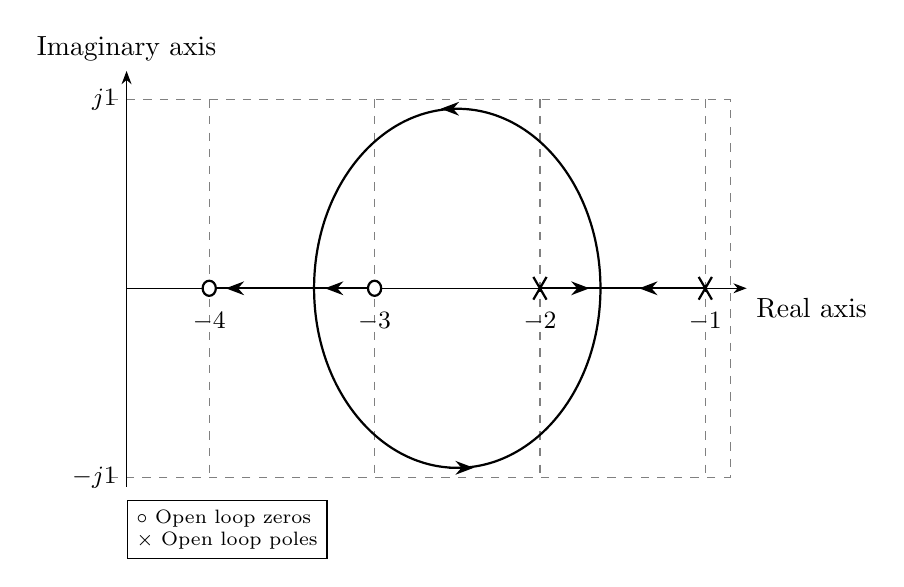
\begin{tikzpicture}[>=Stealth, x=2.1cm, y=2.4cm]
\draw[dashed,gray] (-4.6,1)--(-0.85,1)--(-0.85,-1)--(-4.6,-1);
\draw[dashed,gray] (-4,1)--(-4,-1); \draw[dashed,gray] (-3,1)--(-3,-1); \draw[dashed,gray] (-2,1)--(-2,-1); \draw[dashed,gray] (-1,1)--(-1,-1);
\draw[->] (-4.5,0)--(-0.75,0) node[below right] {Real axis};
\draw[->] (-4.5,-1.05)--(-4.5,1.15) node[above] {Imaginary axis};
\foreach \x in {-4,-3,-2,-1} {\draw (\x,0.02)--(\x,-0.02) node[below=4pt,font=\small] {$\x$};}
\node[left,font=\small] at (-4.5,1) {$j1$}; \node[left,font=\small] at (-4.5,-1) {$-j1$};
% locus on real axis and circle
\draw[thick] (-4,0)--(-3.37,0); \draw[thick] (-3.37,0)--(-3,0);
\draw[thick] (-2,0)--(-1.63,0); \draw[thick] (-1.63,0)--(-1,0);
\draw[thick] (-2.5,0) ellipse (0.866 and 0.95);
\draw[thick,-{Stealth}] (-3.7,0)--(-3.9,0); \draw[thick,-{Stealth}] (-3.15,0)--(-3.3,0);
\draw[thick,-{Stealth}] (-1.8,0)--(-1.7,0); \draw[thick,-{Stealth}] (-1.2,0)--(-1.4,0);
\draw[thick,-{Stealth}] (-2.45,0.95)--(-2.6,0.95); \draw[thick,-{Stealth}] (-2.55,-0.95)--(-2.4,-0.95);
\foreach \p in {-4,-3} {\draw[thick,fill=white] (\p,0) circle (0.04);}
\foreach \p in {-2,-1} {\draw[thick] (\p-0.04,-0.06)--(\p+0.04,0.06) (\p-0.04,0.06)--(\p+0.04,-0.06);}
\node[draw,font=\scriptsize,align=left,anchor=north west,fill=white] at (-4.5,-1.12) {$\circ$ Open loop zeros\\ $\times$ Open loop poles};
\end{tikzpicture}

    \caption{Root locus (ii)}
    \label{fig:EC25-26b}
\end{center}
\end{figure}

%--------------------------------------------------------------- Q27
\item
Let $x[n]$ be a discrete-time signal whose $z$-transform is $X\brak{z}$.

Which of the following statements is/are TRUE?
\hfill (EC~2025)
\begin{enumerate}
    \item The discrete-time Fourier transform (DTFT) of $x[n]$ always exists
    \item The region of convergence (RoC) of $X\brak{z}$ contains neither poles nor zeros
    \item The discrete-time Fourier transform (DTFT) exists if the region of convergence (RoC) contains the unit circle
    \item If $x[n] = \alpha\delta[n]$, where $\delta[n]$ is the unit impulse and $\alpha$ is a scalar, then the region of convergence (RoC) is the entire $z$-plane
\end{enumerate}

%--------------------------------------------------------------- Q28
\item
Consider a message signal $m\brak{t}$ which is bandlimited to $[-W, W]$, where $W$ is in Hz. Consider the following two modulation schemes for the message signal:
\begin{itemize}
    \item Double sideband-suppressed carrier (DSB-SC):
    \begin{align}
    f_{DSB}\brak{t} = A_c\, m\brak{t} \cos\brak{2\pi f_c t}
    \end{align}
    \item Amplitude modulation (AM):
    \begin{align}
    f_{AM}\brak{t} = A_c \brak{1 + \mu\, m\brak{t}} \cos\brak{2\pi f_c t}
    \end{align}
\end{itemize}
Here, $A_c$ and $f_c$ are the amplitude and frequency (in Hz) of the carrier, respectively. In the case of AM, $\mu$ denotes the modulation index.

Consider the following statements:
\begin{enumerate}[label=(\roman*), itemsep=0pt, topsep=2pt]
    \item An envelope detector can be used for demodulation in the DSB-SC scheme if $m\brak{t} > 0$ for all $t$.
    \item An envelope detector can be used for demodulation in the AM scheme \underline{only} if $m\brak{t} > 0$ for all $t$.
\end{enumerate}
Which of the following options is/are correct?
\hfill (EC~2025)
\begin{enumerate}
	\begin{multicols}{2}
    \item (i) is TRUE
    \item (i) is FALSE
    \item (ii) is TRUE
    \item (ii) is FALSE
	\end{multicols}
\end{enumerate}

%--------------------------------------------------------------- Q32
\item
The function $y\brak{t}$ satisfies
\begin{align}
t^2 y''\brak{t} - 2t y'\brak{t} + 2y\brak{t} = 0,
\end{align}
where $y'\brak{t}$ and $y''\brak{t}$ denote the first and second derivatives of $y\brak{t}$, respectively.

Given $y'\brak{0} = 1$ and $y'\brak{1} = -1$, the maximum value of $y\brak{t}$ over $[0, 1]$ is \underline{\hspace{1cm}} (\textit{rounded off to two decimal places}).
\hfill (EC~2025)

%--------------------------------------------------------------- Q33
\item
The generator matrix of a $(6,3)$ binary linear block code is given by
\begin{align}
\vec{G} = \myvec{
1 & 0 & 0 & 1 & 0 & 1 \\
0 & 1 & 0 & 0 & 1 & 1 \\
0 & 0 & 1 & 1 & 1 & 0
}.
\end{align}
The minimum Hamming distance $d_{\min}$ between codewords equals \underline{\hspace{1cm}} (\textit{answer in integer}).
\hfill (EC~2025)

%--------------------------------------------------------------- Q34
\item
All the components in the bandpass filter given below are ideal. The lower $-3$ dB frequency of the filter is 1 MHz.

The upper $-3$ dB frequency (in MHz, \textit{rounded off to the nearest integer}) is \underline{\hspace{1cm}}.
\hfill (EC~2025)
\begin{figure}[H]
\begin{center}
\begin{circuitikz}[american, scale=0.95, transform shape]
\node[op amp] (A) at (7.5,0) {};
\draw (A.-) -- ++(-0.7,0) coordinate (n);
\fill (n) circle(2pt);
\draw (n) to[C, l_=$10C$] ++(-2.2,0) to[R, l_=$R$] ++(-2.2,0) node[left] {$v_S$} ;
\draw (n) -- ++(0,1.3) coordinate (m1) -- ++(0,1.3) coordinate (m2);
\fill (m1) circle(2pt);
\draw (m2) to[R, l=$2R$] (m2 -| A.out);
\draw (m1) to[C, l=$0.1C$] (m1 -| A.out);
\draw (m2 -| A.out) -- (A.out);
\fill (m1 -| A.out) circle(2pt);
\draw (A.+) -- ++(-0.4,0) -- ++(0,-0.5) node[ground] {};
\draw (A.out) to[short, -o] ++(1,0) node[right] {$v_o$};
\end{circuitikz}

    \caption{Bandpass filter}
    \label{fig:EC25-34}
\end{center}
\end{figure}

%--------------------------------------------------------------- Q36
\item
Let $G\brak{s} = \dfrac{1}{10s^2}$ be the transfer function of a second-order system. A controller $M\brak{s}$ is connected to the system $G\brak{s}$ in the configuration shown below.

Consider the following statements.
\begin{enumerate}[label=(\roman*), itemsep=0pt, topsep=2pt]
    \item There exists no controller of the form $M\brak{s} = \dfrac{K_I}{s}$, where $K_I$ is a positive real number, such that the closed loop system is stable.
    \item There exists at least one controller of the form $M\brak{s} = K_P + sK_D$, where $K_P$ and $K_D$ are positive real numbers, such that the closed loop system is stable.
\end{enumerate}
Which one of the following options is correct?
\hfill (EC~2025)
\begin{enumerate}
	\begin{multicols}{2}
    \item (i) is TRUE and (ii) is FALSE
    \item (i) is FALSE and (ii) is TRUE
    \item Both (i) and (ii) are FALSE
    \item Both (i) and (ii) are TRUE
	\end{multicols}
\end{enumerate}
\begin{figure}[H]
\begin{center}
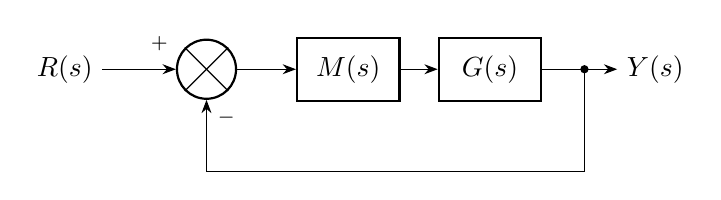
\begin{tikzpicture}[>=Stealth, blk/.style={draw,thick,minimum width=1.3cm,minimum height=0.8cm}]
\node (r) at (0,0) {$R(s)$};
\node[draw,thick,circle,inner sep=0pt,minimum size=0.75cm] (s) at (1.8,0) {};
\draw (s.north west)--(s.south east); \draw (s.north east)--(s.south west);
\node[font=\scriptsize] at (1.2,0.32) {$+$}; \node[font=\scriptsize] at (2.05,-0.62) {$-$};
\node[blk] (m) at (3.6,0) {$M(s)$};
\node[blk] (g) at (5.4,0) {$G(s)$};
\node (y) at (7.5,0) {$Y(s)$};
\draw[->] (r)--(s); \draw[->] (s)--(m); \draw[->] (m)--(g); \draw[->] (g)--(y);
\draw[->] (6.6,0) -- (6.6,-1.3) -- (1.8,-1.3) -- (s.south);
\fill (6.6,0) circle(1.5pt);
\end{tikzpicture}

    \caption{Closed-loop configuration}
    \label{fig:EC25-36}
\end{center}
\end{figure}

%--------------------------------------------------------------- Q37
\item
Consider the polynomial $p\brak{s} = s^5 + 7s^4 + 3s^3 - 33s^2 + 2s - 40$. Let $\brak{L, I, R}$ be defined as follows.
\begin{itemize}
    \item $L$ is the number of roots of $p\brak{s}$ with negative real parts.
    \item $I$ is the number of roots of $p\brak{s}$ that are purely imaginary.
    \item $R$ is the number of roots of $p\brak{s}$ with positive real parts.
\end{itemize}
Which one of the following options is correct?
\hfill (EC~2025)
\begin{enumerate}
	\begin{multicols}{2}
    \item $L = 2,\ I = 2$, and $R = 1$
    \item $L = 3,\ I = 2$, and $R = 0$
    \item $L = 1,\ I = 2$, and $R = 2$
    \item $L = 0,\ I = 4$, and $R = 1$
	\end{multicols}
\end{enumerate}

%--------------------------------------------------------------- Q38
\item
Consider a continuous-time finite-energy signal $f\brak{t}$ whose Fourier transform vanishes outside the frequency interval $[-\omega_c, \omega_c]$, where $\omega_c$ is in rad/sec.

The signal $f\brak{t}$ is uniformly sampled to obtain $y\brak{t} = f\brak{t}\, p\brak{t}$. Here,
\begin{align}
p\brak{t} = \sum_{n=-\infty}^{\infty} \delta\brak{t - \tau - nT_s},
\end{align}
with $\delta\brak{t}$ being the Dirac impulse, $T_s > 0$, and $\tau > 0$. The sampled signal $y\brak{t}$ is passed through an ideal lowpass filter $h\brak{t} = \omega_c T_s \dfrac{\sin\brak{\omega_c t}}{\pi \omega_c t}$ with cutoff frequency $\omega_c$ and passband gain $T_s$.

The output of the filter is given by \underline{\hspace{1cm}}.
\hfill (EC~2025)
\begin{enumerate}
	\begin{multicols}{2}
    \item $f\brak{t}$ if $T_s < \pi/\omega_c$
    \item $f\brak{t - \tau}$ if $T_s < \pi/\omega_c$
    \item $f\brak{t - \tau}$ if $T_s < 2\pi/\omega_c$
    \item $T_s f\brak{t}$ if $T_s < 2\pi/\omega_c$
	\end{multicols}
\end{enumerate}

%--------------------------------------------------------------- Q39
\item
In the circuit below, $M_1$ is an ideal AC voltmeter and $M_2$ is an ideal AC ammeter. The source voltage (in Volts) is $v_s\brak{t} = 100\cos\brak{200t}$.

What should be the value of the variable capacitor $C$ such that the RMS readings on $M_1$ and $M_2$ are 25 V and 5 A, respectively?
\hfill (EC~2025)
\begin{enumerate}
	\begin{multicols}{2}
    \item $25\ \mu$F
    \item $4\ \mu$F
    \item $0.25\ \mu$F
    \item Insufficient information to find $C$
	\end{multicols}
\end{enumerate}
\begin{figure}[H]
\begin{center}
\begin{circuitikz}[american, scale=0.95, transform shape]
\draw (0,0) to[sV, l=$v_s(t)$] (0,3);
\draw (0,3) -- (1.5,3); \draw (0,0) -- (1.5,0);
\draw[thick] (1.5,-0.5) rectangle (3.9,3.5);
\node[align=center] at (2.7,1.5) {Linear\\Time\\Invariant\\Circuit};
\draw (3.9,3) -- (5.3,3); \draw (3.9,0) -- (8.8,0);
\fill (5.3,3) circle(2pt) (5.3,0) circle(2pt);
\draw (5.3,3) to[voltmeter, l_=$M_1$] (5.3,0);
\draw (5.3,3) to[ammeter, l=$M_2$] (7.3,3) -- (8.8,3);
\draw (8.8,3) to[R, l=$5\,\Omega$] (8.8,2.2) to[vC, l=$C$] (8.8,1.4) to[L, l=$1$ H] (8.8,0.4) -- (8.8,0);
\node at (-0.45,2.4) {$+$}; \node at (-0.45,0.6) {$-$};
\node at (4.9,2.2) {$+$}; \node at (4.9,0.8) {$-$};
\end{circuitikz}

    \caption{Circuit with ideal meters}
    \label{fig:EC25-39}
\end{center}
\end{figure}

%--------------------------------------------------------------- Q40
\item
The $Z$-parameter matrix of a two port network relates the port voltages and port currents as follows:
\begin{align}
\myvec{V_1 \\ V_2} = \vec{Z} \myvec{I_1 \\ I_2}
\end{align}
The $Z$-parameter matrix (with each entry in Ohms) of the network shown below is \underline{\hspace{1cm}}.
\hfill (EC~2025)
\begin{enumerate}
	\begin{multicols}{2}
    \item $\myvec{10/3 & 2/3 \\ 2/3 & 10/3}$
    \item $\myvec{2/3 & 10/3 \\ 10/3 & 2/3}$
    \item $\myvec{10 & 2 \\ 2 & 10}$
    \item $\myvec{10/3 & 1/3 \\ 1/3 & 10/3}$
	\end{multicols}
\end{enumerate}
\begin{figure}[H]
\begin{center}
\begin{circuitikz}[american, scale=0.9, transform shape]
\draw (0,2) to[R, l=$2\Omega$, i=$I_1$] (2.5,2) to[R, l=$2\Omega$] (5,2) to[R, l=$2\Omega$, i_<=$I_2$] (7.5,2);
\draw (2.5,2) to[R, l=$2\Omega$] (2.5,0);
\draw (5,2) to[R, l=$2\Omega$] (5,0);
\draw (0,0) -- (7.5,0);
\fill (0,2) circle(2pt) (0,0) circle(2pt) (7.5,2) circle(2pt) (7.5,0) circle(2pt) (2.5,2) circle(1.5pt) (5,2) circle(1.5pt) (2.5,0) circle(1.5pt) (5,0) circle(1.5pt);
\node at (-0.5,1.5) {$+$}; \node at (-0.5,1) {$V_1$}; \node at (-0.5,0.5) {$-$};
\node at (8,1.5) {$+$}; \node at (8,1) {$V_2$}; \node at (8,0.5) {$-$};
\end{circuitikz}

    \caption{Two port network}
    \label{fig:EC25-40}
\end{center}
\end{figure}

%--------------------------------------------------------------- Q41
\item
A source transmits symbol $S$ that takes values uniformly at random from the set $\cbrak{-2, 0, 2}$. The receiver obtains $Y = S + N$, where $N$ is a zero-mean Gaussian random variable independent of $S$. The receiver uses the maximum likelihood decoder to estimate the transmitted symbol $S$.

Suppose the probability of symbol estimation error $P_e$ is expressed as follows:
\begin{align}
P_e = \alpha\, P\brak{N > 1},
\end{align}
where $P\brak{N > 1}$ denotes the probability that $N$ exceeds 1.

What is the value of $\alpha$?
\hfill (EC~2025)
\begin{enumerate}
	\begin{multicols}{4}
    \item $\dfrac{1}{3}$
    \item $1$
    \item $\dfrac{2}{3}$
    \item $\dfrac{4}{3}$
	\end{multicols}
\end{enumerate}

%--------------------------------------------------------------- Q42
\item
Consider a real-valued random process
\begin{align}
f\brak{t} = \sum_{n=1}^{N} a_n\, p\brak{t - nT},
\end{align}
where $T > 0$ and $N$ is a positive integer. Here, $p\brak{t} = 1$ for $t \in [0, 0.5T]$ and $0$ otherwise. The coefficients $a_n$ are pairwise independent, zero-mean unit-variance random variables.

Read the following statements about the random process and choose the correct option.
\begin{enumerate}[label=(\roman*), itemsep=0pt, topsep=2pt]
    \item The mean of the process $f\brak{t}$ is independent of time $t$.
    \item The autocorrelation function $E\sbrak{f\brak{t} f\brak{t + \tau}}$ is independent of time $t$ for all $\tau$.
\end{enumerate}
(Here, $E\sbrak{\cdot}$ is the expectation operation.)
\hfill (EC~2025)
\begin{enumerate}
	\begin{multicols}{2}
    \item (i) is TRUE and (ii) is FALSE
    \item Both (i) and (ii) are TRUE
    \item Both (i) and (ii) are FALSE
    \item (i) is FALSE and (ii) is TRUE
	\end{multicols}
\end{enumerate}

%--------------------------------------------------------------- Q44
\item
A 10-bit analog-to-digital converter (ADC) has a sampling frequency of 1 MHz and a full scale voltage of 3.3 V.

For an input sinusoidal signal with frequency 500 kHz, the maximum SNR (in dB, \textit{rounded off to two decimal places}) and the data rate (in Mbps) at the output of the ADC are \underline{\hspace{1cm}}, respectively.
\hfill (EC~2025)
\begin{enumerate}
	\begin{multicols}{4}
    \item $61.96$ and $10$
    \item $61.96$ and $5$
    \item $33.36$ and $10$
    \item $33.36$ and $5$
	\end{multicols}
\end{enumerate}

%--------------------------------------------------------------- Q45
\item
A positive-edge-triggered sequential circuit is shown below. There are no timing violations in the circuit. Input $P0$ is set to logic `0' and $P1$ is set to logic `1' at all times. The timing diagram of the inputs $SEL$ and $S$ are also shown below.

The sequence of output $Y$ from time $T_0$ to $T_3$ is \underline{\hspace{1cm}}.
\hfill (EC~2025)
\begin{enumerate}
	\begin{multicols}{4}
    \item $1011$
    \item $0100$
    \item $0010$
    \item $1101$
	\end{multicols}
\end{enumerate}
\begin{figure}[H]
\begin{center}
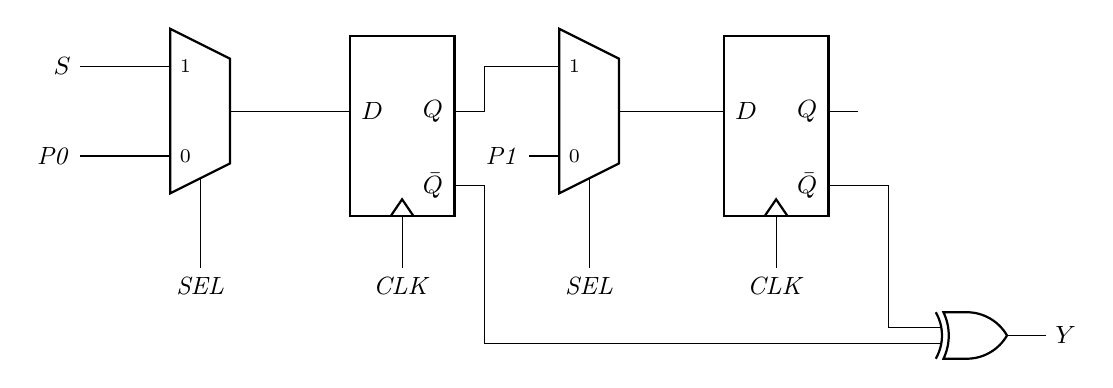
\begin{tikzpicture}[>=Stealth, font=\small, x=0.95cm, y=0.95cm]
% multiplexers
\foreach \mx in {1.2,6.4} {
  \draw[thick] (\mx,1.5)--(\mx+0.8,1.1)--(\mx+0.8,-0.3)--(\mx,-0.7)--cycle;
  \node[font=\scriptsize,right] at (\mx,1.0) {1};
  \node[font=\scriptsize,right] at (\mx,-0.2) {0};
  \draw (\mx+0.4,-0.5) -- (\mx+0.4,-1.7) node[below] {\textit{SEL}};
}
% flip-flops
\foreach \fx in {3.6,8.6} {
  \draw[thick] (\fx,1.4) rectangle (\fx+1.4,-1.0);
  \node[right] at (\fx+0.02,0.4) {$D$};
  \node[left] at (\fx+1.38,0.4) {$Q$};
  \node[left] at (\fx+1.38,-0.6) {$\bar Q$};
  \draw[thick] (\fx+0.55,-1.0)--(\fx+0.7,-0.78)--(\fx+0.85,-1.0);
  \draw (\fx+0.7,-1.0) -- (\fx+0.7,-1.7) node[below] {\textit{CLK}};
}
% inputs of first mux
\node[left] at (0,1.0) {$S$}; \draw (0,1.0)--(1.2,1.0);
\node[left] at (0,-0.2) {\textit{P0}}; \draw (0,-0.2)--(1.2,-0.2);
% mux1 -> FF1
\draw (2.0,0.4)--(3.6,0.4);
% FF1.Q -> mux2 input 1 ;  P1 -> mux2 input 0
\draw (5.0,0.4)--(5.4,0.4)--(5.4,1.0)--(6.4,1.0);
\node[left] at (6.0,-0.2) {\textit{P1}}; \draw (6.0,-0.2)--(6.4,-0.2);
% mux2 -> FF2 ; FF2.Q open
\draw (7.2,0.4)--(8.6,0.4);
\draw (10.0,0.4)--(10.4,0.4);
% XOR
\node[xor gate US, draw, thick, logic gate inputs=nn] (x) at (11.9,-2.6) {};
\draw (10.0,-0.6)--(10.8,-0.6) |- (x.input 1);
\draw (5.0,-0.6)--(5.4,-0.6) |- (x.input 2);
\draw (x.output)--++(0.5,0) node[right] {$Y$};
\end{tikzpicture}

    \caption{Sequential circuit}
    \label{fig:EC25-45a}
\end{center}
\end{figure}
\begin{figure}[H]
\begin{center}
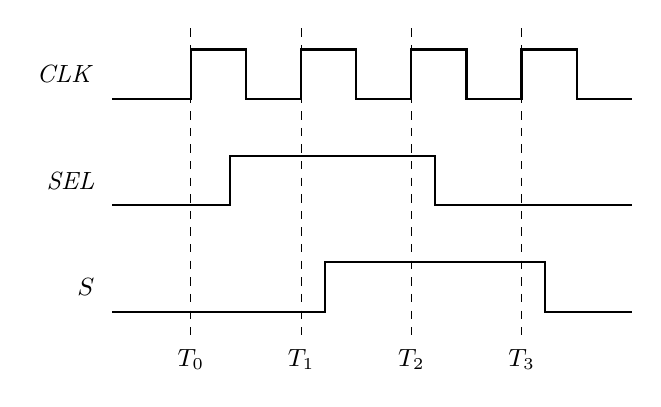
\begin{tikzpicture}[>=Stealth, x=1cm, y=0.9cm, font=\small]
\node[left] at (-0.1,0.35) {\textit{CLK}}; \node[left] at (-0.1,-1.15) {\textit{SEL}}; \node[left] at (-0.1,-2.65) {$S$};
% clock: rising edges at T0..T3 = 1.0, 2.4, 3.8, 5.2
\draw[thick] (0,0)--(1,0)--(1,0.7)--(1.7,0.7)--(1.7,0)--(2.4,0)--(2.4,0.7)--(3.1,0.7)--(3.1,0)--(3.8,0)--(3.8,0.7)--(4.5,0.7)--(4.5,0)--(5.2,0)--(5.2,0.7)--(5.9,0.7)--(5.9,0)--(6.6,0);
% SEL
\draw[thick] (0,-1.5)--(1.5,-1.5)--(1.5,-0.8)--(4.1,-0.8)--(4.1,-1.5)--(6.6,-1.5);
% S
\draw[thick] (0,-3.0)--(2.7,-3.0)--(2.7,-2.3)--(5.5,-2.3)--(5.5,-3.0)--(6.6,-3.0);
\foreach \i/\xx in {0/1.0,1/2.4,2/3.8,3/5.2} {
  \draw[dashed] (\xx,1.0)--(\xx,-3.4);
  \node[below] at (\xx,-3.4) {$T_\i$};
}
\end{tikzpicture}

    \caption{Timing diagram of $CLK$, $SEL$ and $S$}
    \label{fig:EC25-45b}
\end{center}
\end{figure}

%--------------------------------------------------------------- Q49
\item
A square metal sheet of $4\text{ m} \times 4\text{ m}$ is placed on the $x$-$y$ plane as shown in the figure below.

If the surface charge density (in $\mu$C/m$^2$) on the sheet is $\rho_s\brak{x, y} = 4\abs{y}$, then the total charge (in $\mu$C, \textit{rounded off to the nearest integer}) on the sheet is \underline{\hspace{1cm}}.
\hfill (EC~2025)
\begin{enumerate}
	\begin{multicols}{4}
    \item $16$
    \item $85$
    \item $64$
    \item $256$
	\end{multicols}
\end{enumerate}
\begin{figure}[H]
\begin{center}
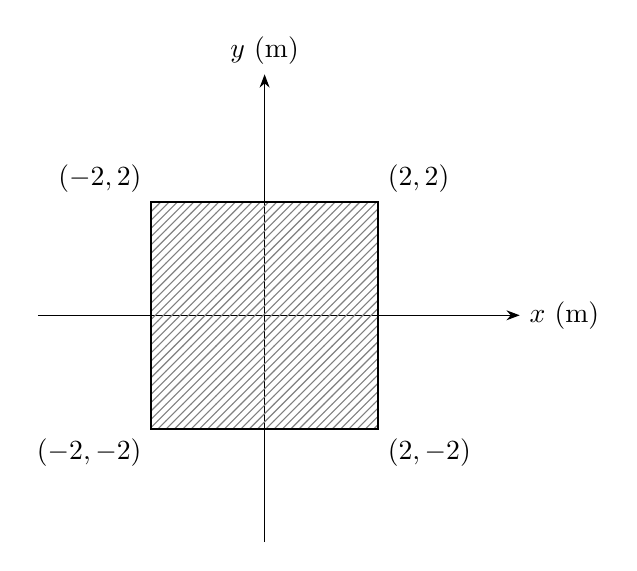
\begin{tikzpicture}[>=Stealth, scale=0.9]
\draw[->] (-3.2,0) -- (3.6,0) node[right] {$x$ (m)};
\draw[->] (0,-3.2) -- (0,3.4) node[above] {$y$ (m)};
\fill[pattern=north east lines, pattern color=gray] (-1.6,-1.6) rectangle (1.6,1.6);
\draw[thick] (-1.6,-1.6) rectangle (1.6,1.6);
\node[above left] at (-1.6,1.6) {$(-2,2)$}; \node[above right] at (1.6,1.6) {$(2,2)$};
\node[below left] at (-1.6,-1.6) {$(-2,-2)$}; \node[below right] at (1.6,-1.6) {$(2,-2)$};
\end{tikzpicture}

    \caption{Square metal sheet}
    \label{fig:EC25-49}
\end{center}
\end{figure}

%--------------------------------------------------------------- Q50
\item
An electric field of 0.01 V/m is applied along the length of a copper wire of circular cross-section with diameter 1 mm. Copper has a conductivity of $5.8 \times 10^7$ S/m.

The current (in Amperes, \textit{rounded off to two decimal places}) flowing through the wire is \underline{\hspace{1cm}}.
\hfill (EC~2025)
\begin{enumerate}
	\begin{multicols}{4}
    \item $0.46$
    \item $1.82$
    \item $0.58$
    \item $1.12$
	\end{multicols}
\end{enumerate}

%--------------------------------------------------------------- Q51
\item
Consider a non-negative function $f\brak{x}$ which is continuous and bounded over the interval $[2, 8]$. Let $M$ and $m$ denote, respectively, the maximum and the minimum values of $f\brak{x}$ over the interval.

Among the combinations of $\alpha$ and $\beta$ given below, choose the one(s) for which the inequality
\begin{align}
\beta \leq \int_{2}^{8} f\brak{x}\, dx \leq \alpha
\end{align}
is guaranteed to hold.
\hfill (EC~2025)
\begin{enumerate}
	\begin{multicols}{2}
    \item $\beta = 5m,\ \alpha = 7M$
    \item $\beta = 6m,\ \alpha = 5M$
    \item $\beta = 7m,\ \alpha = 6M$
    \item $\beta = 7m,\ \alpha = 5M$
	\end{multicols}
\end{enumerate}

%--------------------------------------------------------------- Q52
\item
Which of the following statements involving contour integrals (evaluated counter-clockwise) on the unit circle $C$ in the complex plane is/are TRUE?
\hfill (EC~2025)
\begin{enumerate}
	\begin{multicols}{2}
    \item $\displaystyle\oint_{C} e^{z}\, dz = 0$
    \item $\displaystyle\oint_{C} z^{n}\, dz = 0$, where $n$ is an even integer
    \item $\displaystyle\oint_{C} \cos z\, dz \neq 0$
    \item $\displaystyle\oint_{C} \sec z\, dz \neq 0$
	\end{multicols}
\end{enumerate}

%--------------------------------------------------------------- Q53
\item
Consider a system where $x_1\brak{t}$, $x_2\brak{t}$, and $x_3\brak{t}$ are three internal state signals and $u\brak{t}$ is the input signal. The differential equations governing the system are given by
\begin{align}
\frac{d}{dt}\myvec{x_1\brak{t} \\ x_2\brak{t} \\ x_3\brak{t}} = \myvec{2 & 0 & 0 \\ 0 & -2 & 0 \\ 0 & 0 & 0}\myvec{x_1\brak{t} \\ x_2\brak{t} \\ x_3\brak{t}} + \myvec{1 \\ 1 \\ 1} u\brak{t}.
\end{align}
Which of the following statements is/are TRUE?
\hfill (EC~2025)
\begin{enumerate}
    \item The signals $x_1\brak{t}$, $x_2\brak{t}$, and $x_3\brak{t}$ are bounded for all bounded inputs
    \item There exists a bounded input such that at least one of the signals $x_1\brak{t}$, $x_2\brak{t}$, and $x_3\brak{t}$ is unbounded
    \item There exists a bounded input such that the signals $x_1\brak{t}$, $x_2\brak{t}$, and $x_3\brak{t}$ are unbounded
    \item The signals $x_1\brak{t}$, $x_2\brak{t}$, and $x_3\brak{t}$ are unbounded for all bounded inputs
\end{enumerate}

%--------------------------------------------------------------- Q54
\item
The random variable $X$ takes values in $\cbrak{-1, 0, 1}$ with probabilities
\begin{align}
P\brak{X = -1} = P\brak{X = 1} = \alpha \quad \text{and} \quad P\brak{X = 0} = 1 - 2\alpha, \quad \text{where } 0 < \alpha < \frac{1}{2}.
\end{align}
Let $g\brak{\alpha}$ denote the entropy of $X$ (in bits), parameterized by $\alpha$.

Which of the following statements is/are TRUE?
\hfill (EC~2025)
\begin{enumerate}
	\begin{multicols}{2}
    \item $g\brak{0.4} > g\brak{0.3}$
    \item $g\brak{0.3} > g\brak{0.4}$
    \item $g\brak{0.3} > g\brak{0.25}$
    \item $g\brak{0.25} > g\brak{0.3}$
	\end{multicols}
\end{enumerate}

%--------------------------------------------------------------- Q55
\item
Let $f\brak{t}$ be a periodic signal with fundamental period $T_0 > 0$. Consider the signal $y\brak{t} = f\brak{\alpha t}$, where $\alpha > 1$.

The Fourier series expansions of $f\brak{t}$ and $y\brak{t}$ are given by
\begin{align}
f\brak{t} = \sum_{k=-\infty}^{\infty} c_k\, e^{\j\frac{2\pi}{T_0}kt} \quad \text{and} \quad y\brak{t} = \sum_{k=-\infty}^{\infty} d_k\, e^{\j\frac{2\pi}{T_0}\alpha kt}.
\end{align}
Which of the following statements is/are TRUE?
\hfill (EC~2025)
\begin{enumerate}
    \item $c_k = d_k$ for all $k$
    \item $y\brak{t}$ is periodic with a fundamental period $\alpha T_0$
    \item $c_k = d_k/\alpha$ for all $k$
    \item $y\brak{t}$ is periodic with a fundamental period $T_0/\alpha$
\end{enumerate}

%--------------------------------------------------------------- Q56
\item
Consider a system represented by the block diagram shown below. Which of the following signal flow graphs represent(s) this system? Choose the correct option(s).
\hfill (EC~2025)
\begin{figure}[H]
\begin{center}
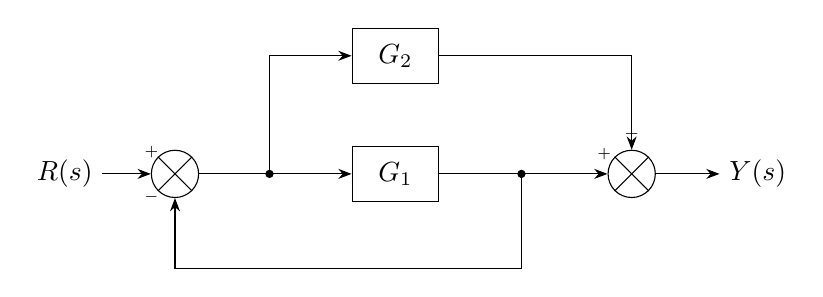
\begin{tikzpicture}[>=Stealth, blk/.style={draw,minimum width=1.1cm,minimum height=0.7cm}, sm/.style={draw,circle,inner sep=0pt,minimum size=0.6cm}]
\node (r) at (0,0) {$R(s)$};
\node[sm] (s1) at (1.4,0) {}; \draw (s1.north west)--(s1.south east); \draw (s1.north east)--(s1.south west);
\node[font=\tiny] at (1.1,0.28) {$+$}; \node[font=\tiny] at (1.1,-0.3) {$-$};
\coordinate (a) at (2.6,0);
\node[blk] (g1) at (4.2,0) {$G_1$};
\coordinate (b) at (5.8,0);
\node[sm] (s2) at (7.2,0) {}; \draw (s2.north west)--(s2.south east); \draw (s2.north east)--(s2.south west);
\node[font=\tiny] at (7.2,0.5) {$+$}; \node[font=\tiny] at (6.85,0.25) {$+$};
\node (y) at (8.8,0) {$Y(s)$};
\node[blk] (g2) at (4.2,1.5) {$G_2$};
\draw[->] (r)--(s1); \draw (s1)--(a); \draw[->] (a)--(g1); \draw (g1)--(b); \draw[->] (b)--(s2); \draw[->] (s2)--(y);
\fill (a) circle(1.5pt) (b) circle(1.5pt);
\draw[->] (a) |- (g2); \draw[->] (g2) -| (s2.north);
\draw[->] (b) -- (5.8,-1.2) -| (s1.south);
\end{tikzpicture}

    \caption{Block diagram}
    \label{fig:EC25-56}
\end{center}
\end{figure}
\begin{enumerate}
	\begin{multicols}{2}
    \item 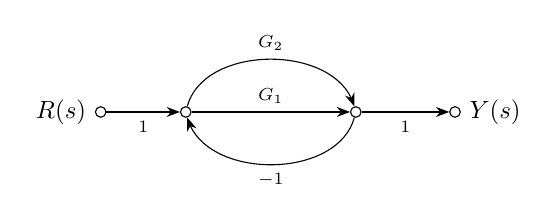
\begin{tikzpicture}[>=Stealth, baseline=(current bounding box.center), scale=0.9, transform shape, sfn/.style={draw,circle,inner sep=1.5pt}, lab/.style={font=\scriptsize}]
\node[sfn,label=left:{$R(s)$}] (r) at (0,0) {}; \node[sfn] (a) at (1.2,0) {}; \node[sfn] (b) at (3.6,0) {}; \node[sfn,label=right:{$Y(s)$}] (y) at (5.0,0) {};
\draw[->] (r)--(a) node[midway,below,lab] {$1$};
\draw[->] (a)--(b) node[pos=0.5,above,lab] {$G_1$};
\draw[->] (a) to[bend left=75] node[above,lab] {$G_2$} (b);
\draw[->] (b) to[bend left=75] node[below,lab] {$-1$} (a);
\draw[->] (b)--(y) node[midway,below,lab] {$1$};
\end{tikzpicture}

    \item 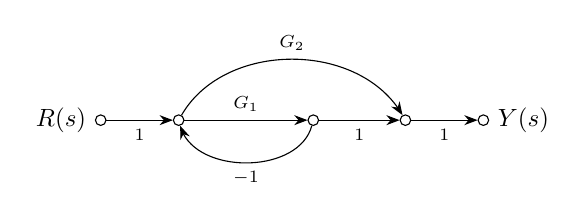
\begin{tikzpicture}[>=Stealth, baseline=(current bounding box.center), scale=0.9, transform shape, sfn/.style={draw,circle,inner sep=1.5pt}, lab/.style={font=\scriptsize}]
\node[sfn,label=left:{$R(s)$}] (r) at (0,0) {}; \node[sfn] (a) at (1.1,0) {}; \node[sfn] (m) at (3.0,0) {}; \node[sfn] (c) at (4.3,0) {}; \node[sfn,label=right:{$Y(s)$}] (y) at (5.4,0) {};
\draw[->] (r)--(a) node[midway,below,lab] {$1$};
\draw[->] (a)--(m) node[pos=0.5,above,lab] {$G_1$};
\draw[->] (m)--(c) node[midway,below,lab] {$1$};
\draw[->] (c)--(y) node[midway,below,lab] {$1$};
\draw[->] (a) to[bend left=60] node[above,lab] {$G_2$} (c);
\draw[->] (m) to[bend left=75] node[below,lab] {$-1$} (a);
\end{tikzpicture}

    \item 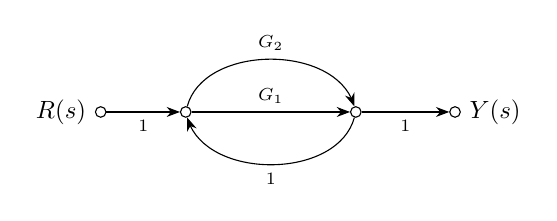
\begin{tikzpicture}[>=Stealth, baseline=(current bounding box.center), scale=0.9, transform shape, sfn/.style={draw,circle,inner sep=1.5pt}, lab/.style={font=\scriptsize}]
\node[sfn,label=left:{$R(s)$}] (r) at (0,0) {}; \node[sfn] (a) at (1.2,0) {}; \node[sfn] (b) at (3.6,0) {}; \node[sfn,label=right:{$Y(s)$}] (y) at (5.0,0) {};
\draw[->] (r)--(a) node[midway,below,lab] {$1$};
\draw[->] (a)--(b) node[pos=0.5,above,lab] {$G_1$};
\draw[->] (a) to[bend left=75] node[above,lab] {$G_2$} (b);
\draw[->] (b) to[bend left=75] node[below,lab] {$1$} (a);
\draw[->] (b)--(y) node[midway,below,lab] {$1$};
\end{tikzpicture}

    \item 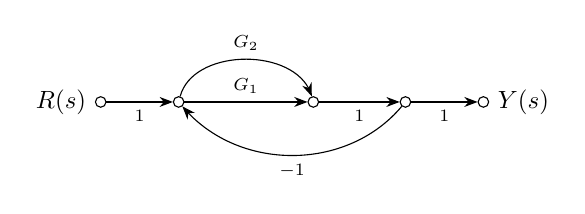
\begin{tikzpicture}[>=Stealth, baseline=(current bounding box.center), scale=0.9, transform shape, sfn/.style={draw,circle,inner sep=1.5pt}, lab/.style={font=\scriptsize}]
\node[sfn,label=left:{$R(s)$}] (r) at (0,0) {}; \node[sfn] (a) at (1.1,0) {}; \node[sfn] (b) at (3.0,0) {}; \node[sfn] (c) at (4.3,0) {}; \node[sfn,label=right:{$Y(s)$}] (y) at (5.4,0) {};
\draw[->] (r)--(a) node[midway,below,lab] {$1$};
\draw[->] (a)--(b) node[pos=0.5,above,lab] {$G_1$};
\draw[->] (b)--(c) node[midway,below,lab] {$1$};
\draw[->] (c)--(y) node[midway,below,lab] {$1$};
\draw[->] (a) to[bend left=75] node[above,lab] {$G_2$} (b);
\draw[->] (c) to[bend left=50] node[below,lab] {$-1$} (a);
\end{tikzpicture}

	\end{multicols}
\end{enumerate}

%--------------------------------------------------------------- Q58
\item
Two fair dice (with faces labeled 1, 2, 3, 4, 5, and 6) are rolled. Let the random variable $X$ denote the sum of the outcomes obtained.

The expectation of $X$ is \underline{\hspace{1cm}} (\textit{rounded off to two decimal places}).
\hfill (EC~2025)

%--------------------------------------------------------------- Q59
\item
Consider the vectors
\begin{align}
\vec{a} = \myvec{1 \\ 1}, \qquad \vec{b} = \myvec{0 \\ 3\sqrt{2}}.
\end{align}
For real-valued scalar variable $x$, the value of
\begin{align}
\min_{x} \norm{\vec{a}x - \vec{b}}_2
\end{align}
is \underline{\hspace{1cm}} (\textit{rounded off to two decimal places}).

$\norm{\cdot}_2$ denotes the Euclidean norm, i.e., for $\vec{y} = \myvec{y_1 \\ y_2}$, $\norm{\vec{y}}_2 = \sqrt{y_1^2 + y_2^2}$.
\hfill (EC~2025)

%--------------------------------------------------------------- Q60
\item
$X$ and $Y$ are Bernoulli random variables taking values in $\cbrak{0, 1}$. The joint probability mass function of the random variables is given by:
\begin{align}
\begin{split}
P\brak{X = 0, Y = 0} &= 0.06 \\
P\brak{X = 0, Y = 1} &= 0.14 \\
P\brak{X = 1, Y = 0} &= 0.24 \\
P\brak{X = 1, Y = 1} &= 0.56
\end{split}
\end{align}
The mutual information $I\brak{X; Y}$ is \underline{\hspace{1cm}} (\textit{rounded off to two decimal places}).
\hfill (EC~2025)

%--------------------------------------------------------------- Q61
\item
The diode in the circuit shown below is ideal. The input voltage (in Volts) is given by $V_I = 10 \sin 100\pi t$, where time $t$ is in seconds.

The time duration (in ms, \textit{rounded off to two decimal places}) for which the diode is forward biased during one period of the input is \underline{\hspace{1cm}}.
\hfill (EC~2025)
\begin{figure}[H]
\begin{center}
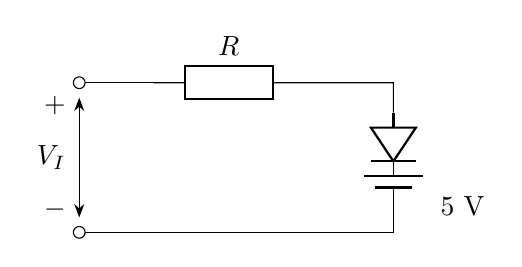
\begin{tikzpicture}[>=Stealth, scale=0.95]
\draw (0,2) node[circle,draw,inner sep=1.5pt,fill=white] {} -- (1,2);
\draw (1,2) to[generic, l=$R$] (3,2) -- (4.2,2) -- (4.2,1.6);
\draw[thick] (4.2,1.6) -- (4.2,1.4); \draw[thick] (3.9,1.4) -- (4.5,1.4) -- (4.2,0.95) -- cycle; \draw[thick] (3.9,0.95) -- (4.5,0.95);
\draw (4.2,0.95) -- (4.2,0.75); \draw[thick] (3.8,0.75) -- (4.6,0.75); \draw[thick] (3.95,0.6) -- (4.45,0.6);
\draw (4.2,0.6) -- (4.2,0) -- (0,0) node[circle,draw,inner sep=1.5pt,fill=white] {};
\node[right] at (4.7,0.35) {$5$ V};
\draw[<->] (0,0.2)--(0,1.8); \node[left] at (-0.05,1.0) {$V_I$}; \node[left] at (-0.05,1.7) {$+$}; \node[left] at (-0.05,0.3) {$-$};
\end{tikzpicture}

    \caption{Diode circuit}
    \label{fig:EC25-61}
\end{center}
\end{figure}

%--------------------------------------------------------------- Q62
\item
In the circuit shown below, the AND gate has a propagation delay of 1 ns. The edge-triggered flip-flops have a set-up time of 2 ns, a hold-time of 0 ns, and a clock-to-Q delay of 2 ns.

The maximum clock frequency (in MHz, \textit{rounded off to the nearest integer}) such that there are no setup violations is \underline{\hspace{1cm}}.
\hfill (EC~2025)
\begin{figure}[H]
\begin{center}
\begin{tikzpicture}[>=Stealth, font=\small, ff/.style={draw,minimum width=1.3cm,minimum height=1.7cm}]
\node[ff] (f1) at (0,0) {}; \node[ff] (f2) at (3,0) {};
\foreach \f in {f1,f2} {\node[right] at ($(\f.west)+(0.02,0.45)$) {$D$}; \node[left] at ($(\f.east)+(-0.02,0.45)$) {$Q$}; \node[left] at ($(\f.east)+(-0.02,-0.45)$) {$\bar Q$};
 \draw ($(\f.south)+(-0.15,0)$)--($(\f.south)+(0,0.2)$)--($(\f.south)+(0.15,0)$);}
\node[and gate US,draw,logic gate inputs=nn,anchor=input 1] (a) at (5.2,0.45) {};
\draw ($(f1.east)+(0,0.45)$) -- ($(f2.west)+(0,0.45)$);
\draw ($(f2.east)+(0,0.45)$) -- (a.input 1);
\node (X) at (4.3,-0.6) {$X$}; \draw (X.east) -| (a.input 2);
\draw (a.output) -- ++(0.5,0) |- (0,1.8) -| (-1.2,0.45) -- ($(f1.west)+(0,0.45)$);
\draw (f1.south) -- ++(0,-0.7) coordinate (c1); \draw (f2.south) -- ++(0,-0.7) coordinate (c2);
\draw (c1) -- (c2); \fill ($(c1)!0.5!(c2)$) circle(1.5pt) -- ++(0,-0.4) node[below] {$CLK$};
\end{tikzpicture}

    \caption{Flip-flops with AND gate}
    \label{fig:EC25-62}
\end{center}
\end{figure}

%--------------------------------------------------------------- Q65
\item
Two resistors are connected in a circuit loop of area $5\text{ m}^2$, as shown in the figure below. The circuit loop is placed on the $x$-$y$ plane.

When a time-varying magnetic flux, with flux-density $B\brak{t} = 0.5t$ (in Tesla), is applied along the positive $z$-axis, the magnitude of current $I$ (in Amperes, \textit{rounded off to two decimal places}) in the loop is \underline{\hspace{1cm}}.
\hfill (EC~2025)
\begin{figure}[H]
\begin{center}
\begin{circuitikz}[american, scale=1.0, transform shape]
\fill[pattern=north west lines, pattern color=gray!60] (0,0) rectangle (3.4,2.4);
\draw[thick] (0,0) -- (3.4,0) -- (3.4,0.45) to[R, l_=$2\,\Omega$] (3.4,1.65) -- (3.4,2.4);
\draw[thick, -{Stealth}] (3.4,2.4) -- (1.9,2.4) node[above,pos=0.5] {$I$};
\draw[thick] (1.9,2.4) -- (0,2.4) -- (0,1.65) to[R, l_=$2\,\Omega$] (0,0.45) -- (0,0);
\draw[thick, -{Stealth}, bend left=40] (1.3,-0.8) to (1.0,0.15);
\node at (0.7,-1.0) {\large Loop Area};
% axes
\draw[dashed,thick,-{Stealth}] (5.6,1.2)--(5.6,2.5) node[right] {$y$};
\draw[dashed,thick,-{Stealth}] (5.6,1.2)--(7.2,1.2) node[right] {$x$};
\draw[dashed,thick,-{Stealth}] (5.6,1.2)--(4.9,0.6) node[below left] {$z$};
\end{circuitikz}

    \caption{Circuit loop in a time-varying magnetic field}
    \label{fig:EC25-65}
\end{center}
\end{figure}
\end{enumerate}


\end{document}
